\section{
    Effect of uniform relative motions on the Rheology at finite Reynolds number. 
    }
\label{sec:particle_def}


Preceding studies have intended to model the rheology of dilute emulsion of neutrally buoyant deformable droplets, in stokes regime \citep{goddard1967nonlinear,lhuillier1987phenomenology,maffettone1998equation}.
More recently, researchers have been trying to include inertial effects in these models \citet{raja2010inertial,mwasame2018macroscopic}. 
However, these studies have been conducted with the objective of determining the response to the mean shearing motion of a neutrally buoyant suspension on the stress, i.e. they study the mean stress $\bm{\sigma}$ in terms of the imposed flow gradient $\textbf{E}_f$ for a given microstructure. 
To the knowledge of the author all preceding study disregards the impact of relative motion, that we denote $\textbf{u}_{fp} = \textbf{u}_f - \textbf{u}_p$, on the suspension rheology.
We recall that $\textbf{u}_{p f} = \textbf{u}_p  - \textbf{u}_f$ is the relative averaged velocity of the droplet minus that of the carrier fluid.


In this section we make use of the \textit{hybrid model} derived in the preceding sections to demonstrate what is the effect of uniform phase relative motion on the Rheology at finite Reynolds number. 
As this problem is rather complicated we first use some simplifying hypotheses. 
We start by considering only uniform relative motion. 
Indeed, as the purpose is to point out the effect of the relative translational motions on the stress, we consider that there is no mean shear within the emulsion, i.e. $\textbf{E}_f = 0$. 
As discussed in the preceding section we consider that the droplet shape relaxes instantaneously with the ambient fluid motion, in other words we consider that the deformation of the drops are in quasi-steady state regime with the solicitation of the flow. 
Finally, as stated in the beginning of this chapter we only focus on small deformations.  



To introduce the problem we first present a way to compute analytically the droplet deformation in terms of its relative motion with the carrier phase. 
Indeed, it is shown with the help of the reciprocal theorem that the closure term of \ref{eq:dev} can be obtained at $\mathcal{O}(Re \phi)$.
Doing so we obtain an explicit formula for the droplet deformation. 
We deduce from this application that at a finite Reynolds number, the first moment of the hydrodynamic forces is  part of the cause of the droplet deformation and acts as a source term inside the mean carrier fluid stress. 
Therefore, in the second step, we expose a completely closed formulation of the bulk stress of the carrier fluid phase. 


The particle averaged linear momentum and mass conservation, can be obtained carrying the same procedure as in \ref{chap:daniel1} and yield the same as for non-deformable particles. 
Only the closure terms of the latter equations will be influenced by considering the drop shape and orientation.
The same comments can be made regarding the carrier phase equations. 
This implies that the equations used in \ref{chap:daniel1} are still valid upon having the right closure terms. 
Consequently, for a mono-disperse suspension, these equations provide an equation for the mean particle phase velocity $\textbf{u}_p$ fluid velocity $\textbf{u}_f$ and particle volume fraction $\phi_f$ or $\phi_d$. 
Thus, in the next paragraphs, we will consider these variables as known variables. 

\subsection{Determination of the averaged particle shape}

In \ref{sec:local_eq_ellipse} we have seen that in the quasi-steady state regime the rate of strain equation, i.e. the equation for $\textbf{E}_\alpha$, reduces directly to an equation for the particle shape $\bm\chi_p$. 
Thus, we will use \ref{sec:local_eq_ellipse} to compute the averaged particle shape. 
Applying the average operator on \ref{eq:steady} yields,
\begin{equation}
    (\bm\chi_{p})_{ij}
    = 
    \frac{5}{4}Ca \left[
        (\textbf{F}_p^h )_{ij}
        + \zeta Re (\textbf{F}_p^{vv})_{ij}
        +    \lambda (\textbf{F}_p^{\sigma})_{ij}
    \right],
    \label{eq:steady_state_avg}
\end{equation}
where we introduced, $n_p \textbf{F}_p^h = \pavg{\textbf{F}_\alpha^h}$ and so on. 
Thus, in this regime, one might be able to compute the instantaneous averaged shape of the particle upon the knowledge of the mean surface stress distribution, $\textbf{F}_p^h$, the mean particle's internal shear stress tensor, $\textbf{F}_p^{\sigma}$, and finally, the mean particle internal inertial contribution $\textbf{F}_p^{vv}$. 

As the purpose of this section is to determine the effect of relative motion on the shape of the particles, we will consider only the portion of the closures that are functions of $\textbf{u}_{pf}$, which is the relative phase velocity. 

\subsubsection{Discussion on the closure problem}   

However, to broaden our understanding, we first propose to discus what form the right-hand side of \ref{eq:steady_state_avg} may take in the simplest scenario. 
Only for this subsection we consider a mean shear rate $\textbf{E}_f$ since it is useful for the subsequent discussion. 

Let us first discuss the term $\textbf{F}^{vv}$. 
It is clear that a complete closure for this term taking into account all parameters at hand is impossible. 
Nevertheless, as shown in \ref{ap:reciprocal} we may already compute this term assuming only the translation of a spherical droplet in a pure linear stokes flow. 
As this term is inertial by nature, its computation from the stokes flow solution just gives us the first order in $Re$ accurate term.
Thus, for $Re \zeta < 1$, $Ca = 0$ and $\phi = 0$ we may write,
\begin{align}
    \textbf{F}^{vv}_p
    % &= 
    % \intO{\rho_d [\textbf{v}_d^0  \textbf{v}_d^0  - \frac{1}{3}\rho_d (\textbf{v}_d^0 \cdot \textbf{v}_d^0)\bm\delta]}\\
    = \frac{\rho_d \phi_d}{20(\lambda +1 )^2}
    \left[
        \textbf{u}_{p f}\textbf{u}_{p f} 
    -\frac{1}{3} (\textbf{u}_{p f}\cdot \textbf{u}_{p f})\bm\delta
    % + 7\pavg{\textbf{u}_\alpha'\textbf{u}_\alpha'}/n_p 
    % + 2k_p \bm\delta
    \right]
    + \frac{\rho_d \phi_d a^2}{21 (\lambda + 1)^2}[\textbf{E}_f\cdot \textbf{E}_f - \frac{1}{3}(\textbf{E}:\textbf{E})\bm\delta]
    + \mathcal{O}((Re\zeta)^2,Ca, \phi)
    \label{eq:vv_closure}
\end{align}
This closure is valid solely for spherical particles at first order in $Re$. 
Thus, as soon as the particle deforms an additional correction must be provided to account for this deformation. 
Notice that these corrections can be obtained at low but finite capillary number $Ca$, from \citet{leal2007advanced} for a droplet immersed in pure linear flows, and \citet{taylor1964deformation} for a droplet in relative translation. 
Indeed, these authors provide the detailed velocity fields of such cases. 
Anyhow, we would like to point out that due to the presence of $\textbf{u}_{\alpha f}$ in \ref{eq:vv_closure} the internal droplets motions, $\textbf{v}_d^0$, induce a coupling between the droplets translational motion $\textbf{u}_\alpha$ and deformation $\bm\chi_\alpha$ through \ref{eq:dev_dim}. 
As could be expected, the fluid phase shear rate $\textbf{E}_f$ also induces an internal motion (see \ref{fig:flowlines}), which when accounting for the particle inertia plays a role in the dynamical shape balance.  
To conclude, notice that $\textbf{F}^{vv}$ is the only reason why the density ratio $\zeta$ comes into play when computing the steady-state shape of a droplet (for example see \citet{taylor1964deformation}). 

The internal particle shear rate forcing term $\textbf{F}^\sigma$, also plays an important role in the shape dynamics. 
Applying the previous reasoning we obtain a first glimpse of the functional form of this term. 
Indeed, from \ref{ap:reciprocal} we found that, 
\begin{equation*}
    \textbf{F}_p^{\sigma}
    % = - \mu_d \intS{(\textbf{n}_i \textbf{v}_{d,j}^0 + \textbf{n}_j \textbf{v}_{d,i}^0)}
    = \mu_d \phi \frac{ 2 }{\lambda+1}
    \textbf{E}_f
    + \mathcal{O}(Re,Ca,\phi). 
\end{equation*}
In this situation notice the absence of $\textbf{u}_{fp}$ in the expression.
This because the translation of a droplet in stokes flow does not alter the shape of the droplets. 
Nevertheless, at $\mathcal{O}(Re^2)$ it is reasonable to expect the emergence of terms proportional to $\textbf{u}_{fp}$ in the expression.
Approximately the same treatment can be adopted for the external stress contribution $\textbf{F}^h$. 
Indeed, it is found that, 
\begin{equation}
    % \pavg{\intS{\textbf{r}\bm{\sigma}_f^0 \cdot \textbf{n}_d}} 
    \textbf{F}^h_p
    = 
    \frac{3}{5}\mu_f \phi_d \left(\frac{2+5\lambda}{1+\lambda}\right)
    \textbf{E}_f
    + \mathcal{O}(Re,Ca,\phi).
    \label{eq:closure_stress}
\end{equation}
Again at the next order in $Re$ it is likely that the translation of the droplet might contribute to this term. 
Again a coupling between deformation and particle translation. 
Nevertheless, under this form, the closure problem is incomplete as \ref{eq:dev} requires to compute the closure term with an accuracy of $\mathcal{O}(Ca)$ at least. 
Notice that in \citet{raja2010inertial} they give the next order in $Ca$ for this term.


Overall, we have shown that these closure terms can indeed be expressed as a combination of particles and carrier fluid properties.
Particularly, we demonstrated that there is an explicit link between deformation and translational velocity of the particle at finite $Re$, through the term $\textbf{F}^{vv}_p$. 
% Overall, we have shown that these closures could be expressed based on the singularity solution of stokes flows. 
Thus, it is clear that the relative velocity plays a role only at finite Reynolds numbers. 
Indeed, at $Re = 0$ only the mean fluid shear rate $\textbf{E}_f$ is present in the source terms, $\textbf{F}^h_p$ and $\textbf{F}_p^{\sigma}$. 
Therefore, as our objective is to determine the effect of relative motion on the shape of the particle, we decided to compute the closure terms at $\mathcal{O}(Re)$. 
Indeed, at finite $Re$ it will eventually make appear the relation of these closures with the relative motion $\textbf{u}_{pf}$. 


\subsubsection{Determination of the closure terms at first order in $Re$}

To determine the $\mathcal{O}(Re)$ correction of $\textbf{F}_p$ the closure terms of we first expand the RHS of \ref{eq:steady_state_avg} in at Taylor expansion about $Re = 0$. 
We obtain the following relation, 
\begin{align*}
    \textbf{F}_p(Re)
    = 
    \textbf{F}_p^{(0)}
    + Re\textbf{F}_p^{(1)}
    + \ldots 
    = 
    [(\textbf{F}^h_p)^{(0)}+\lambda (\textbf{F}^\sigma_p)^{(0)}]
    + Re[(\textbf{F}^h_p)^{(1)}+\lambda (\textbf{F}^\sigma_p)^{(1)}+\zeta (\textbf{F}^{vv}_p)^{(0)}]
    + \ldots 
\end{align*}
where the terms with superscript $^{(0)}$ correspond to the adequate stokes flow solution, and the terms with $^{(1)}$, to the first inertial correction solution. 
It is interesting to notice that to be accurate at the first order in $Re$ we only need to compute the term $(\textbf{F}^{vv}_p)^{(0)}$.
In other words, this term is the integral of the particle's internal velocity for a translating sphere in stokes flow.  
Indeed, as we are interested only in the particle relative translation we can already obtain this term from \ref{eq:vv_closure} and show that, 
\begin{equation}
    (\textbf{F}^{vv}_p)^{(0)}
    % &= 
    % \intO{\rho_d [\textbf{v}_d^0  \textbf{v}_d^0  - \frac{1}{3}\rho_d (\textbf{v}_d^0 \cdot \textbf{v}_d^0)\bm\delta]}\\
    = \frac{1}{20(\lambda +1 )^2}
        [\textbf{u}_{p f}\textbf{u}_{p f} 
    -\frac{1}{3} (\textbf{u}_{p f}\cdot \textbf{u}_{p f})\bm\delta]. 
    % + 7\pavg{\textbf{u}_\alpha'\textbf{u}_\alpha'}/n_p 
    % + 2k_p \bm\delta
    \label{eq:closure_vv}
\end{equation}
Regarding the term $(\textbf{F}^h_p)^{(1)}$ and $\lambda (\textbf{F}^\sigma_p)^{(1)}$, the calculation becomes more complicated since it requires the solution at first order accuracy in $Re$ for the fields $\bm\sigma_f^{(1)}$ and $\textbf{u}_f^{(1)}$. 

Based on an original proof given in \ref{ap:reciprocal} we demonstrate how to compute $(\textbf{F}^h_p)^{(1)}$ and $\lambda (\textbf{F}^\sigma_p)^{(1)}$. 
The method is based on the reciprocal theorem, following the strategy used in \citet{stone2001inertial} for solid particles. 
% for finite $Re$ and is not limited to the context presented here.
Specifically in \ref{ap:reciprocal} we show how to compute the first order correction in $\mathcal{O}(Re)$ of any moment of hydrodynamic forces on the surface of a spherical droplet immersed in an arbitrary flows. 
While this general derivation can be of interest in numerous other problems, for our purposes, we focus specifically on deriving the closure terms present in \ref{eq:vv_closure} under the assumption of uniform relative motion between particles and carrier fluid. 
We show that the computation of $(\textbf{F}^h_p)^{(1)}$, independently of $\lambda (\textbf{F}^\sigma_p)^{(1)}$ were not possible, however we could demonstrate  how to compute the sum of these terms. 

We could show with the reciprocal theorem that the first order correction of the internal particle stresses is identically null, meaning $(\textbf{F}^\sigma_p)^{(1)} = 0$. 
This can be explained by noticing that the velocity fields $\textbf{u}_k$ of a droplet in translation follows stokes equation close to the particle, even when considering a first order correction in $Re$.
In other world $\textbf{u}^{(1)}_d =0 $ thus,  $(\textbf{F}^\sigma_p)^{(1)} = 0$. 

Regarding the traceless and symmetric part of the first moment of hydrodynamic forces we obtained, 
\begin{align}
    (\textbf{F}^h_p)^{(1)}  
    % + \lambda (\textbf{F}^\sigma_p)^{(1)}
    &=
    - C_1 v_p
    [
        \textbf{u}_{pf}\textbf{u}_{pf} - \frac{1}{3}(\textbf{u}_{pf}\cdot \textbf{u}_{pf})\bm\delta 
    ]\\
    C_1 &=
    % \frac{345 \lambda^{3} + 928 \lambda^{2} + 856 \lambda + 272}{320 \left(\lambda + 1\right)^{3}}
    % + \frac{\zeta \left(12 \lambda + 13\right)}{20 \left(\lambda + 1\right)^{2}}
    \frac{57 \lambda^{3} + 114 \lambda^{2} + 80 \lambda + 20}{80 \left(\lambda + 1\right)^{3}}
    % \intS{\textbf{u}_f^{(1)}\cdot  \hat{\bm\sigma}_f \cdot \textbf{n}}
    % \intOf{\textbf{u}_f^{(0)}\cdot ( \div \hat{\bm\sigma}_f)}
    \label{eq:closure_sigma_e}
\end{align}
% This, proves indirectly that the Stresslet on a drop in translation is not null at finite $Re$.
where $v_p$ is the averaged volume of the particles, here $v_p = 4/3 \pi a^3$.  
Thus, a translating droplet experiences a non-zero first moment of the hydrodynamic forces due to the inertial effects of the surrounding fluid. This result indicates that the stress distribution over the surface of the particle is unbalanced, which, as we will see, leads to particle deformation.
This contrasts with the Stokes flow case, where the hydrodynamic stress is balanced, as we've observed that $(\textbf{F}^h_p)^{(0)} = 0$ when considering only relative translation.  
Notice that this derivation is based on spherical droplets' solution. 
Thus, they are only accurate at zeroth order in  $\mathcal{O}(|\bm\chi|)$. 


Using \ref{eq:closure_vv} and \ref{eq:closure_sigma_e} in  \ref{eq:steady_state_avg}, the deformation of the droplet can be estimated at $\mathcal{O}(Re^{2/3},Ca,\phi)$ and yields, 
\begin{align*}
    (\bm\chi_{p})_{ij}
    &= 
    \frac{5}{4}We \left[
        (\textbf{F}_p^h )_{ij}^{(1)}
        + \lambda (\textbf{F}_p^{\sigma})_{ij}^{(1)}
        + \zeta (\textbf{F}_p^{vv})_{ij}^{(0)}
    \right]\\
    &= We \beta [\textbf{u}_{pf}\textbf{u}_{pf} - \frac{1}{3}(\textbf{u}_{pf}\cdot \textbf{u}_{pf})\bm\delta ]
    + \mathcal{O}(Re^{3/2},\phi,Ca),
\end{align*}
with, 
\begin{equation*}
    \beta = 
    + \frac{57 \lambda^{3} + 114 \lambda^{2} + 80 \lambda + 20}{64 \left(\lambda + 1\right)^{3}}
    + \frac{\zeta}{16 \left(\lambda + 1\right)} 
\end{equation*}
where we have introduced the \textit{Weber} number $We = Re \cdot Ca$. 
Notice that $\beta < 0$ $\forall \lambda,\zeta$, which means that the droplet will eventually deform into an oblate ellipsoid.
This conclusion align with \citet{taylor1964deformation} even if the coefficient $\beta$ corresponding to $2\zeta$ in their  study does not correspond exactly.   

Let us now discuss the physical implication of the droplet deformation. 
If the droplet deform, this means that the local forces above and below the droplet are stronger than the forces on the sides of the droplets. 
If the droplet experience this distribution of forces on their surfaces, this means that the continuous phase experience an equal, but opposite in sign distribution of forces from the surface of the droplets. 
Consequently, the average carrier fluid phase stress will be impacted by the non-vanishing value of $\textbf{F}^h_p$ as well. 
% Thus, in the next section we compute the relative importance of $\textbf{F}^h_p$ on the carrier phase stress. 

% \subsection{Determination of the bulk stress}

% Rhetorical studies are most of the time carried in the purpose of finding out the expression of the stress in terms of the mean fluid phase shear. 
% In other world one is trying to find out the \textit{bulk stress} response from a mean shearing motion. 
% As we did not consider a mean shear rate in this study, our objective is to determine the \textit{bulk stress} induced by relative translating motions between phases.  

% A first part of the awnser is provided by the expression of the second moments of the hydrodynamic forces, 
% which we now reads, 
% \begin{equation}
%     \pSavg{\textbf{rr}(\bm\sigma\cdot \textbf{n})}
%     \sim \textbf{u}_{pf} \bm\delta.
% \end{equation}
% Nevertheless, this expression could not be carrier to the next order in $Re$. 
% Therefore, to stay consistent we dismiss this term by considering a homogeneous suspension of droplets, in which case the inhomogeneous terms vanish.
% In this situation we may write the equivalent homogeneous \textit{bulk} stress as, 
% \begin{equation*}
%     \bm{\sigma}_m^\text{ed}
%     = 
%     \avg{\rho^0\textbf{u}_m'\textbf{u}'_m}
%     + \phi_fp_f\bm\delta
%     - 2\mu_f\textbf{e}  
%     + \pOavg{(\bm{\sigma}_d^0 - 2\mu_f \textbf{e}_d^0)}
%     % - \phi_d(\bm{\sigma}_d - 2\mu_f \textbf{e}_d)
%     + \pSavg{\bm\sigma_I^0}. 
%     \label{eq:bulk_stress_translating}
% \end{equation*} 
% Notice that since we only consider relative translation the term $2 \mu_f \textbf{e}$ usually present, doesn't appears. 
% As discussed in the preceding chapter $\avg{\rho^0\textbf{u}_m'\textbf{u}'_m}$ is the pseudo-turbulent stress. 

% The second term on the right-hand side of \ref{eq:bulk_stress_translating} represent the fluid phase pressure, it is considered as an unknown and therefore does not need to be reformulated. 
% The third term, represents the particle internal stresses, usually we use the first moment of momentum balance to reformulate this term as surface integral of the fluid phase stress. 
% Nevertheless, in this context as we know exactly the particle stress constitutive relation we may write, 
% \begin{equation*}
%     \pOavg{(\bm\sigma_{d,ij}^0 -2\mu_f \textbf{e}_{d,ij}^0)}
%     =
%     - \pOavg{p_d^0} \bm\delta_{ij}
%     +2 \mu_f (\lambda - 1) \phi_d \textbf{E}_{p,ij}
%     + \mu_f (\lambda - 1) \pSavg{(\textbf{n}_i \textbf{v}_{d,j}^0 + \textbf{n}_j \textbf{v}_{d,i}^0)}
%     % - \mu_f  \pSavg{(\textbf{n}_i \textbf{v}_{d,j}^0 + \textbf{n}_j \textbf{v}_{d,i}^0)}
% \end{equation*} 
% Then the last term of \ref{eq:bulk_stress_translating} is the surface tension stress which we see is expressible as, 
% \begin{equation*}
%     \pSavg{\bm\sigma_{I,ij}^0}
%     = \frac{\gamma \phi_d }{a} \left[
%         2\bm\delta_{ij} 
%         + \frac{4  }{5} \bm\chi_{p,ij}
%     \right]
% \end{equation*}
% Including all these expressions into the bulk stress leads to, 
% \begin{align*}
%     \bm{\sigma}_m^\text{ed}
%     = 
%     \avg{\rho^0\textbf{u}_m'\textbf{u}'_m}
%     + \left[
%         \phi_fp_f
%         - \pOavg{p_d^0}
%         +\frac{2 \gamma \phi_d }{a}
%     \right]\bm\delta
%     - 2\mu_f\textbf{e}
%     + 2 \mu_f (\lambda - 1) \phi_d \textbf{E}_{p,ij}\\
%     + \mu_f (\lambda - 1) \pSavg{(\textbf{n}_i \textbf{v}_{d,j}^0 + \textbf{n}_j \textbf{v}_{d,i}^0)}
%     % - \phi_d(\bm{\sigma}_d - 2\mu_f \textbf{e}_d)
%     +  \frac{4 \gamma \phi_d }{5 a} \bm\chi_{p,ij}
% \end{align*} 
% Notice that the terms within the bracts are all isotropic, meaning that they represent an effective pressure to the suspension, while the others terms are all symmetric traceless tensors. 
% Additionally, the presence of $\bm\chi_{p,ij}$ represents the elastic contribution of the particles. 
% In other worlds the suspension becomes visco-elastic in this regime. 
% To complete this expression one must solve \ref{eq:avg_chi_I} and \ref{eq:avg_E_I}, the orientation equations \eqref{eq:dt_Ap}. 
% Additionally, as the pressure of the particle phase appears explicitly in the equation, one may use \ref{eq:dt_trM2} which can be reformulated as, 
% \begin{equation*}
% % -  \bm\Gamma_{\alpha,ml}\bm\Gamma_{\alpha,mk} \textbf{M}_{\alpha,kl}  
% \frac{2\gamma \phi_d }{a} 
% - \pOavg{p_d^0} 
% = 
% \frac{1}{3}\pSavg{\textbf{r}_m\cdot\bm\sigma_{1,mk}^0\cdot \textbf{n}_k} 
% + \frac{1}{3}\pOavg{\rho_2 \textbf{v}_{d,m}^0\cdot \textbf{v}_{d,m}^0}. 
% \end{equation*}
% It is also possible to combine all these pressure term and solve for the sum of it. 


% \tb{Discus more this point on  a point of view phenomenological o not speak closures}
% \tb{make the link with the system of equation ? }


\subsection{The continuous phase stress}

In this section, we would like to compare the relative influence of the first moment of the hydrodynamic forces due to relative translating motions, to the other contributions present in the continuous phase equivalent stresses. 
For the comparison to be meaningful $\textbf{F}^h_p$ must be compared to other stresses proportional to $\sim [\textbf{u}_{fp}\textbf{u}_{fp}-\frac{1}{3}(\textbf{u}_{fp}\cdot\textbf{u}_{fp})\bm\delta]$. 
Notice that in 1D models, for example, the absence of mean shear is inherently assumed, making it essential to discuss the impact of relative translation on the mean stress of the continuous phase. 
Indeed, in such scenarios, terms proportional to the relative motions become the only contributions to the carrier phase stress. 

Now that the motivation are properly stated let us present the expression of the homogeneous averaged continuous phase stress, namely,
\begin{equation}
    \bm{\sigma}^\text{eq}_f = 
    \phi_f p_f \bm\delta 
    % - 2\mu_f \textbf{e} 
    +\avg{\rho_f\chi_f\textbf{u}_f'\textbf{u}_f'}
    % - \pSavg{\textbf{r}\times(\bm{\sigma}_f^0\cdot \textbf{n}_d)}
    % \\
    - \pSavg{\textbf{r}\bm{\sigma}_f^0\cdot \textbf{n}_d}
    + 2 \mu_f \pOavg{\textbf{e}_d^0}
    % \\
    % + \div \left[
    %     \frac{1}{2} \pSavg{\textbf{rr}\bm{\sigma}_f^0\cdot \textbf{n}_d}
    %     - 2 \mu_f\pOavg{ \textbf{re}_d^0 }
    %     + \ldots
    % \right]
    \label{eq:sigma_eq_f}
\end{equation} 
Again the mean shear rate $2\mu_f\textbf{e}$, usually present in this expression, does not appear since we are concerned with only relative motion and no macroscopic shear. 
Likewise, the higher order moment of the hydrodynamic force are not proportional to $\textbf{u}_{fp}$ or $\textbf{u}_{fp}\textbf{u}_{fp}$ since they appear under the divergence operator (see \ref{chap:daniel2}), we therefore neglected them. 
Under this form it is clear that the mean carrier fluid stress is generated due to the competitive action of the mean continuous phase pressure, the \textit{Reynolds stress} tensor, and the \textit{Stresslet} tensor. 
As one can see the deformation of the droplets described by $\bm\chi_p$ as well as their rate of strain $\textbf{E}_p$ do not appear explicitly in the equivalent stress. 
However, that does not mean that they do not play a role in the average stress. 
Indeed, since the exchange term in \ref{eq:sigma_eq_f} can be substituted using \ref{eq:dt_S} making appears explicitly those quantities witnessing their importance. 
Nevertheless, as it has been shown, in the steady state regime we obtained algebraic expressions for $\bm\chi_p$ and neglected $\textbf{E}_p$. 
This means that in this context we may rather directly find a closure for the \textit{Stresslet} and \textit{Reynolds stress} tensor in terms of the particles and carrier fluid properties. 
Since we only assume relative and uniform motion, closing \ref{eq:sigma_eq_f} means that we must find the relation of these closures with relative mean motion.

In the most general scenario one would solve an equation for $\textbf{u}_p$, $\textbf{u}_f$, $\bm\chi_p$, $\textbf{E}_p$ and, upon having the right closures, he would compute the stress based on this potential expression. 
In the limit of the dilute regime, meaning that we neglect all terms $\sim \mathcal{O}(\phi^2)$ or higher, and only considering relative translational motions, these closures can be determined. 
As we will show in a subsequent chapter the \textit{Reynolds stress} tensor can be closed in the steady state homogeneous dilute regime and yields, 
\begin{equation}
    \avg{\rho_f\chi_f\textbf{u}_f'\textbf{u}'_f}
    = Re  \phi C_{Re}^1 \left[
        \textbf{u}_{pf}
        \textbf{u}_{pf}
        -\frac{1}{3}
        (\textbf{u}_{pf}
        \cdot\textbf{u}_{pf})\bm\delta
    \right]
    + Re \phi C_{Re}^2 (\textbf{u}_{pf}\cdot\textbf{u}_{pf}) \bm\delta, 
    \label{eq:Reynolds_stress}
\end{equation}
where, 
\begin{align*}
    C_{Re}^1(\phi,\lambda)
    = \frac{1}{20(1+l)^2}\left[
        \frac{9(2+3\lambda)^2}{4}\Gamma(1/3) \phi^{-1/3}
        - (27+82\lambda +62\lambda^2)
    \right],\\
    C_{Re}^2(\phi,\lambda)
    = \frac{1}{6(1+l)^2}\left[
        \frac{(2+3\lambda)^2}{4}\Gamma(1/3) \phi^{-1/3}
        - (3+10\lambda +8\lambda^2)
    \right],
\end{align*}
Notice that the constant $C_{Re}^2$ and $C_{Re}^1$ are still function of $\phi$ due to the non-linear relation of $\avg{\rho_f\chi_f\textbf{u}_f'\textbf{u}'_f}$ with the volume fraction. 
Additionally, we have decomposed the right-hand side terms of \ref{eq:Reynolds_stress}, such that the first term, proportional to $C_{Re}^1$, corresponds to a traceless symmetric tensor, and the second term proportional to $C_{Re}^2$, represents the isotropic contribution.  

The \textit{Stresslet term} has been derived in \ref{ap:reciprocal}. 
As discussed in the latter section, it is shown that the zeroth order $Re$ term is identically null. 
However, when first-order inertial effects are considered then we have (see \ref{ap:reciprocal}),
\begin{equation*}
    \pSavg{\textbf{r}\bm{\sigma}_f^0 \cdot \textbf{n}_d}
    - 2 \mu_f \pOavg{\textbf{e}_d^0}
    =
    - \phi Re C_1
    [
        \textbf{u}_{pf}\textbf{u}_{pf} - \frac{1}{3}(\textbf{u}_{pf}\cdot \textbf{u}_{pf})\bm\delta 
    ]
    + Re \phi C_2 (\textbf{u}_{pf}\cdot \textbf{u}_{pf}) 
    + \phi p_f \bm\delta
    \label{eq:stresslet_trans}
\end{equation*} 
where the constant $C_1$ is shown to be exactly the same as in \ref{eq:closure_sigma_e} and the constant $C_2 =\frac{3\lambda^2 + 6\lambda + 4}{48(\lambda +1 )^2}$ as shown in \ref{ap:reciprocal}. 
In the same way as for the \textit{Reynolds stress} term, we have decomposed the \textit{Stresslet} into an isotropic and symmetric traceless tensor, proportional to $C_2$ and $C_1$, respectively. 
Notice that in opposition to \ref{eq:Reynolds_stress}, $C_1$ and $C_2$ are not functions of the volume fraction for the \textit{Stresslet} term. 

Making use of \ref{eq:Reynolds_stress} and \ref{eq:stresslet_trans} inside \ref{eq:sigma_eq_f} yields the following formula for the carrier fluid averaged stress, 
\begin{multline*}
    \bm{\sigma}^\text{eq}_f = 
    \left[ p_f + Re \phi  [C_{Re}^2(\phi,\lambda) + C_2(\lambda)](\textbf{u}_{pf}\cdot \textbf{u}_{pf}) \right]\bm\delta \\
    % - 2\mu_f \textbf{e} 
    % +\avg{\rho_f\chi_f\textbf{u}_f'\textbf{u}_f'} \\
    + Re \phi [C_{Re}^1(\phi,\lambda) + C_1(\lambda)]\left[
            \textbf{u}_{pf}\textbf{u}_{pf}
            - \frac{1}{3}(\textbf{u}_{pf}\cdot \textbf{u}_{pf})\bm\delta
    \right]
    + \mathcal{O}(Re^{3/2},\phi^2, Ca^2 ).
    \label{eq:stress_closed}
\end{multline*} 
We note that the terms on the first line on the right-hand side of \ref{eq:stress_closed} correspond to an equivalent pressure term, consisting of:  
(1) The mean hydrostatic pressure of the carrier fluid $p_f$, 
(2) the isotropic contribution from the \textit{Reynolds stress}, and 
(3) the isotropic part of the \textit{Stresslet}, the latter two contribution being proportional to $Re \phi (\textbf{u}_{fp}\cdot \textbf{u}_{fp})$.  
The terms on the second line represent the effective symmetric and traceless part of the carrier phase stress. 
This term arises entirely from the relative motion between the particles and the carrier fluid. 



Overall, at steady state equilibrium and for uniform relative motion the stress is driven by two distinct physical contributions: 
(1) the \textit{Reynolds stress}, also called the particle induced turbulence. 
(2) the \textit{Stresslet} tensor which is also proportional to these two parameters. 
Notice that the particle-induced turbulence is well known term. 
Even though the closure provided here is new, many studies already tackled this issue to model this term in the case of relative motion between phases with solid particles. 
The latter contribution, however, is often taken into account when mean shearing motions are considered, (with \ref{eq:closure_stress} for example), indeed, this term is the cause of the well-known Einstein viscosity. 
However, the value of this term in the presence of relative phase velocity, see \ref{eq:stresslet_trans},  and at $\mathcal{O}(Re)$, have been completely overlooked in the literature. 
Therefore, the presence of this term in the stress constitutive equation \eqref{eq:stress_closed}  is new and seems to have been ignored up to now. 
For these reasons, we now evaluate the relative importance of the \textit{Reynolds stress} often used in this context compared to the \textit{Stresslet} term. 

\begin{figure}
    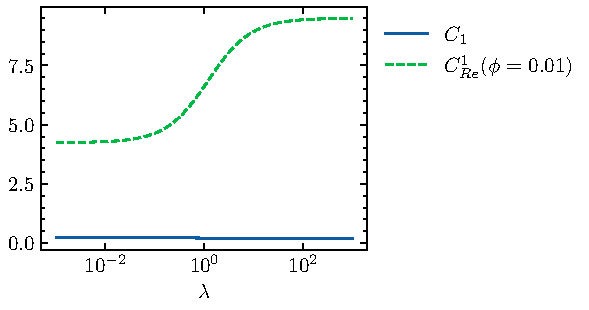
\includegraphics[height=0.25\textwidth]{image/Theory/C1.pdf}
    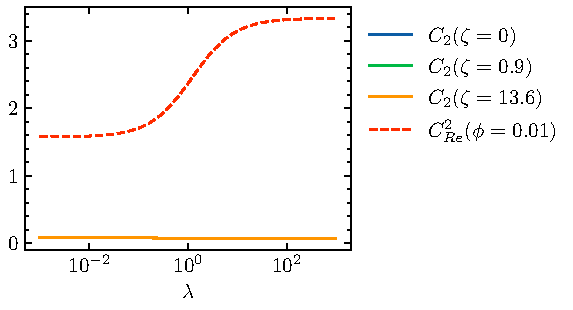
\includegraphics[height=0.25\textwidth]{image/Theory/C2.pdf}
    \caption{
    (solid lines) Values based on \ref{eq:stresslet_trans} of the constant $C_1$ (left)  and $C_2$ (right) in terms of the viscosity ratio $\lambda$.
    (dashed lines) Values based on \ref{eq:Reynolds_stress} of the constant $C_1^{Re}$ (left) and $C_2^{Re}$ (right)  evaluated at $\phi = 0.05$ in terms of the viscosity ratio $\lambda$.
    }
    \label{fig:relative_comparaison}
\end{figure}
Since, $C_1^{Re} \& C_2^{Re} \sim \phi^{-1/3}$ we may already conclude that the $C_1^{Re} \ll C_1$ and $C_2^{Re} \ll C_2$ when $\phi \to 0$. 
This, means that for very low volume fraction the \textit{Stresslet} term  is in fact completely negligible. 
What about higher volume fraction ? 
Since our solution is derived in the dilute limit it seems reasonable to compare the values of the \textit{Reynolds stress} and the \textit{Stresslet} at a maximum value of $\phi = 0.05$. 

% In \ref{fig:relative_comparaison} (right) we compare the vectical contribution of the \textit{Stresslet} and \textit{Reynolds stress} at $\phi =0.05$. 
% By vertical, we mean in the direction of the relative motions. 
% % In this situation we compare the constants $C = \frac{2}{3} C_1 +C_2$ and $C_Re =\frac{2}{3} C_{Re}^1 + C_{Re}^2$ to take in account the total contribution of both stresses in the direction of $\textbf{u}_{fp}$.  
% We can observe that the constant $C_{Re} < C$ regardless of the viscosity ratio $\lambda$. 
% Consequently, the isotropic part of the \textit{Stresslet} due to relative translational motion is less important than the induced pseudo-turbulence.
% However, it still represents a non-negligible part of the stress when $\lambda = 0$ (bubbles in water) where $C_{Re}^2$ is minimum and $C_2$ maximum. 


In \ref{fig:relative_comparaison} (right) we compare the isotropic contribution of the \textit{Stresslet} and \textit{Reynolds stress} at $\phi =0.05$. 
We can observe that the constant $C_{Re}^2 < C_2$ regardless of the viscosity ratio $\lambda$. 
Consequently, the isotropic part of the \textit{Stresslet} due to relative translational motion is less important than the induced pseudo-turbulence.
However, it still represents a non-negligible part of the stress when $\lambda = 0$ where $C_{Re}^2$ is minimum and $C_2$ maximum. 


In \ref{fig:relative_comparaison} (left) we compare the symmetric traceless contribution of the \textit{Stresslet} at $\phi =0.05$. 
% Before, doing so let us analysis the behavior of the \textit{Stresslet} in terms of $\zeta$ and $\lambda$ independently of the \textit{Reynolds stress}. 
% These density ratios correspond to respectively, a drop of mercury in water $\zeta = 13.6$, a droplet of oil in water $\zeta = 0.9$ and a bubble in water $\zeta = 0$. 
% We can observe that $C_1(\zeta = 13.9)=C_1(\zeta = 0.9)=C_1(\zeta = 0)$ when $\lambda \to \infty$.
% Consequently, in the low inertia regime the density ratio $\zeta$ doesn't impact the \textit{Stresslet} term. 
% This is consistent with the quasi-steady state assumption adopted to derive these closures. 
At low $\lambda$ we observe that $C_1$ decrease. 
% Notice that a droplet of mercury in water has $\lambda =1$, thus this limit the realistic value that $C_1$ can take, i.e. a heavy droplet with $\lambda = 0$ might probably not exist. 
% Now let us turns our attention to the \textit{Reynolds stress} contribution. 
We can observe as earlier on \ref{fig:relative_comparaison} (right) that $C_{Re}^1$ and $C_{Re}^2$ decrease for low viscosity ratio. 
This simply means that bubbles induce less velocity fluctuation than solid particles when being in steady translational motion in the fluid. 
This is easily explained by acknowledging that the fluid slip on the bubbles' surface while it follows exactly the surface of a solid sphere, inducing more wakes. 
As witnessed by \ref{fig:relative_comparaison} (left) the \textit{Stresslet} term is comparable, but still lower than the \textit{Reynolds stress} term.
Indeed, at $\lambda = 0$ $C_1 \approx 0.3$ while $C^1_{Re} \approx 1.9$, we may conclude that this contribution is negligible for bubbles.
However, at $\lambda \to \infty$ we observe that $C_1 \approx 0.8$ and $C^1_{Re}\approx 4$ meaning that the \textit{Stresslet} is $20\%$ of the total stress, which might be negligible.  

Overall, we conclude that in this regime where the two competitive contributions to the mean carrier phase stress are the \textit{Reynolds stress} and the \textit{Stresslet} term, the latter cannot be neglected for $\lambda \to \infty$ even tough being lower than the former. 
Additionally, when one considers bubble ($\lambda=0$) it seems that the contribution of the stress is negligible. 
Regarding the isotropic part of the \textit{Stresslet} it cannot be neglected for all $\lambda$, however, both contributions have to be compared to the hydrostatic pressure to determine their relevance. 